


\thispagestyle{empty}
\mbox{}
\vfill
\begin{center}
    \textit{This page is left intentionally blank.}
\end{center}
\vfill
\newpage
\noindent


\begin{multicols}{2}

\noindent
---\textbf{System}---\textbf{Threads:} Hardware threads (CPU cores) each
may run one software thread (program) at a time. Switching,
between threads is context switching (overhead). E.g.,
Go manages internal thread pools, offering it to the OS,
reducing overhead.
\textbf{Thread Comm:} Inter-process communication (IPC), 
threads communicate via shared memory (e.g., channels, pipes, virtual memory).
\textbf{Conc. \& Parrelism:} Concurrency shuffles tasks,
parallelism runs tasks simultaneously (threads).
\textbf{Dist. Conn:} A client connects to a server (client-server model), a TCP conn. (FIFO)
secures the line, the RPC (remote procedure call) abstracts
dist. communication.
\textbf{Races \& Deadlocks:} Data race, two threads manipulating shared data (reads-onlys are fine).
\textbf{Mutexes:} Placing locks around shared data, stopping concurrent access.
\textbf{RPC Fail Models:} At-least-once, client retries until a response is received.
Rads are fine, writes cause race conditions. At-most-once, server handles dupes, clients
send unique IDs (cached responses). Exactly-once, both at-least-once and at-most-once.
\textbf{(a)sync:} Asynchronous, non-blocking, no waiting for a response. Synchronous, blocking, waiting for a response.
\textbf{(un)buffered-channers:} Unbuffered, sender waits for receiver on some thread to receive message. Buffered, sender sends message(s) to a buffer, takes one at a time.
\textbf{Task, Data, Pipeline Parallelism:} Task, same data, different tasks. Data, same task, different data. Pipeline, task split into dependent stages, independent stages run in parallel.
\textbf{Time Accr:} Physical clocks drift due to hardware limitations. Atomic clocks, have insignificant drift. NTP (network time protocol), 
utilizes GPS satellites to sync time, to a ground truth clocks, which propagates time to other systems.
---\textbf{Logical Time}---\textbf{Lamport Clocks:} 
Lamport Clocks, $(t_p, p)$, $t_p$ time of process $p$, monotonically increases for each event/send (Total Ordering). 
Receivers $q$ resolve time differences, $t_q = max((t_p+1), t_q)$ (send vs. local time). Given 
two events $a$ \& $b$, timestamps $t(a)$ \& $t(b)$, with $r$ trace: $a\to_r b \implies t(a) < t(b)$ (causal ordering);
$t(a) \geq t(b) \implies a \not\to_r b$ (concurrent); $(t(a) = t(b) \land a\gg b) \implies a \to_r b$, s.t., ($\gg$) rep. process order.
\textbf{Non-causal:} $(a\ll b):= (a \not\to_r b) \land (b\not\to_r a)$ (concurrent).
\textbf{Vector Clocks:} Operate as an array of Lamport clocks, index is process $p_i$, and value is $t_{p_i}$ (time); However, sends do not increment $t_{p_i}$.
Given timestamps $a$ \& $b$, if all indexes in $a$ are larger than $b$, $a\to_r b$. If some in $a$ are larger than $b$, vice versa, $a<>b$ (non-comparable, concurrent, partial ordering).

\noindent
TaskPar. DataPar. PipePar. La\&Ve.Clock:
\noindent
\rule{\linewidth}{0.4pt}\\
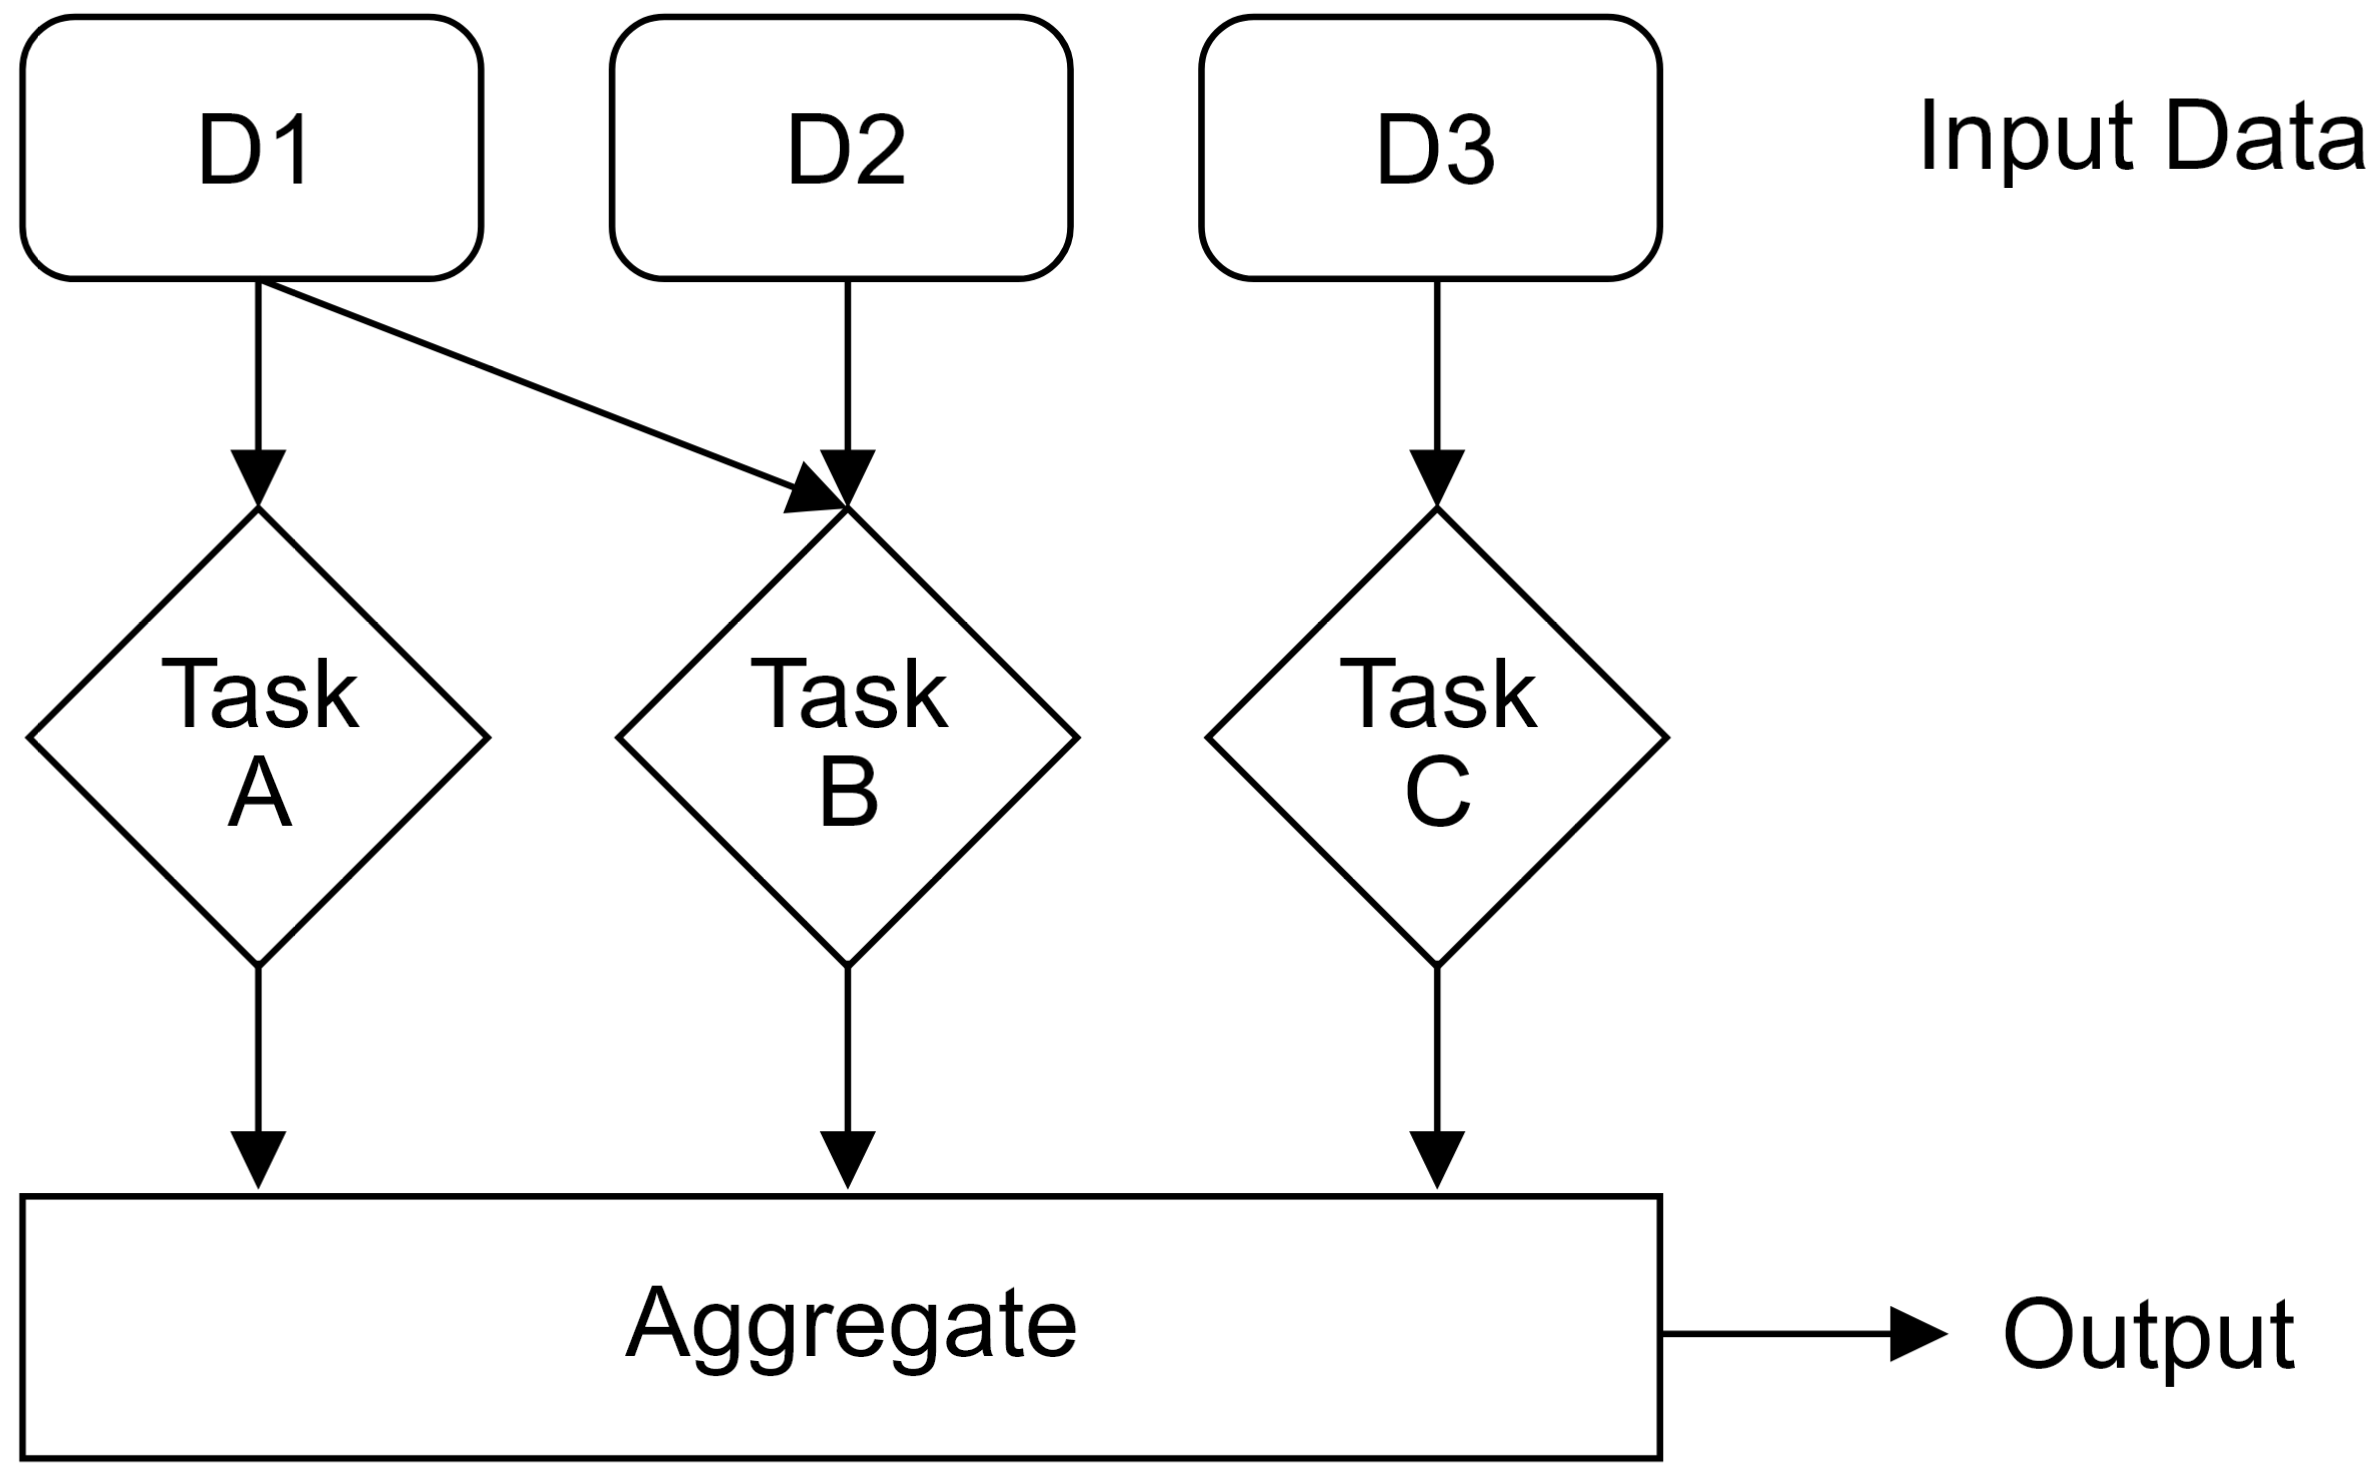
\includegraphics[width=.5\linewidth]{./Sections/rpc_2/tpar.png}
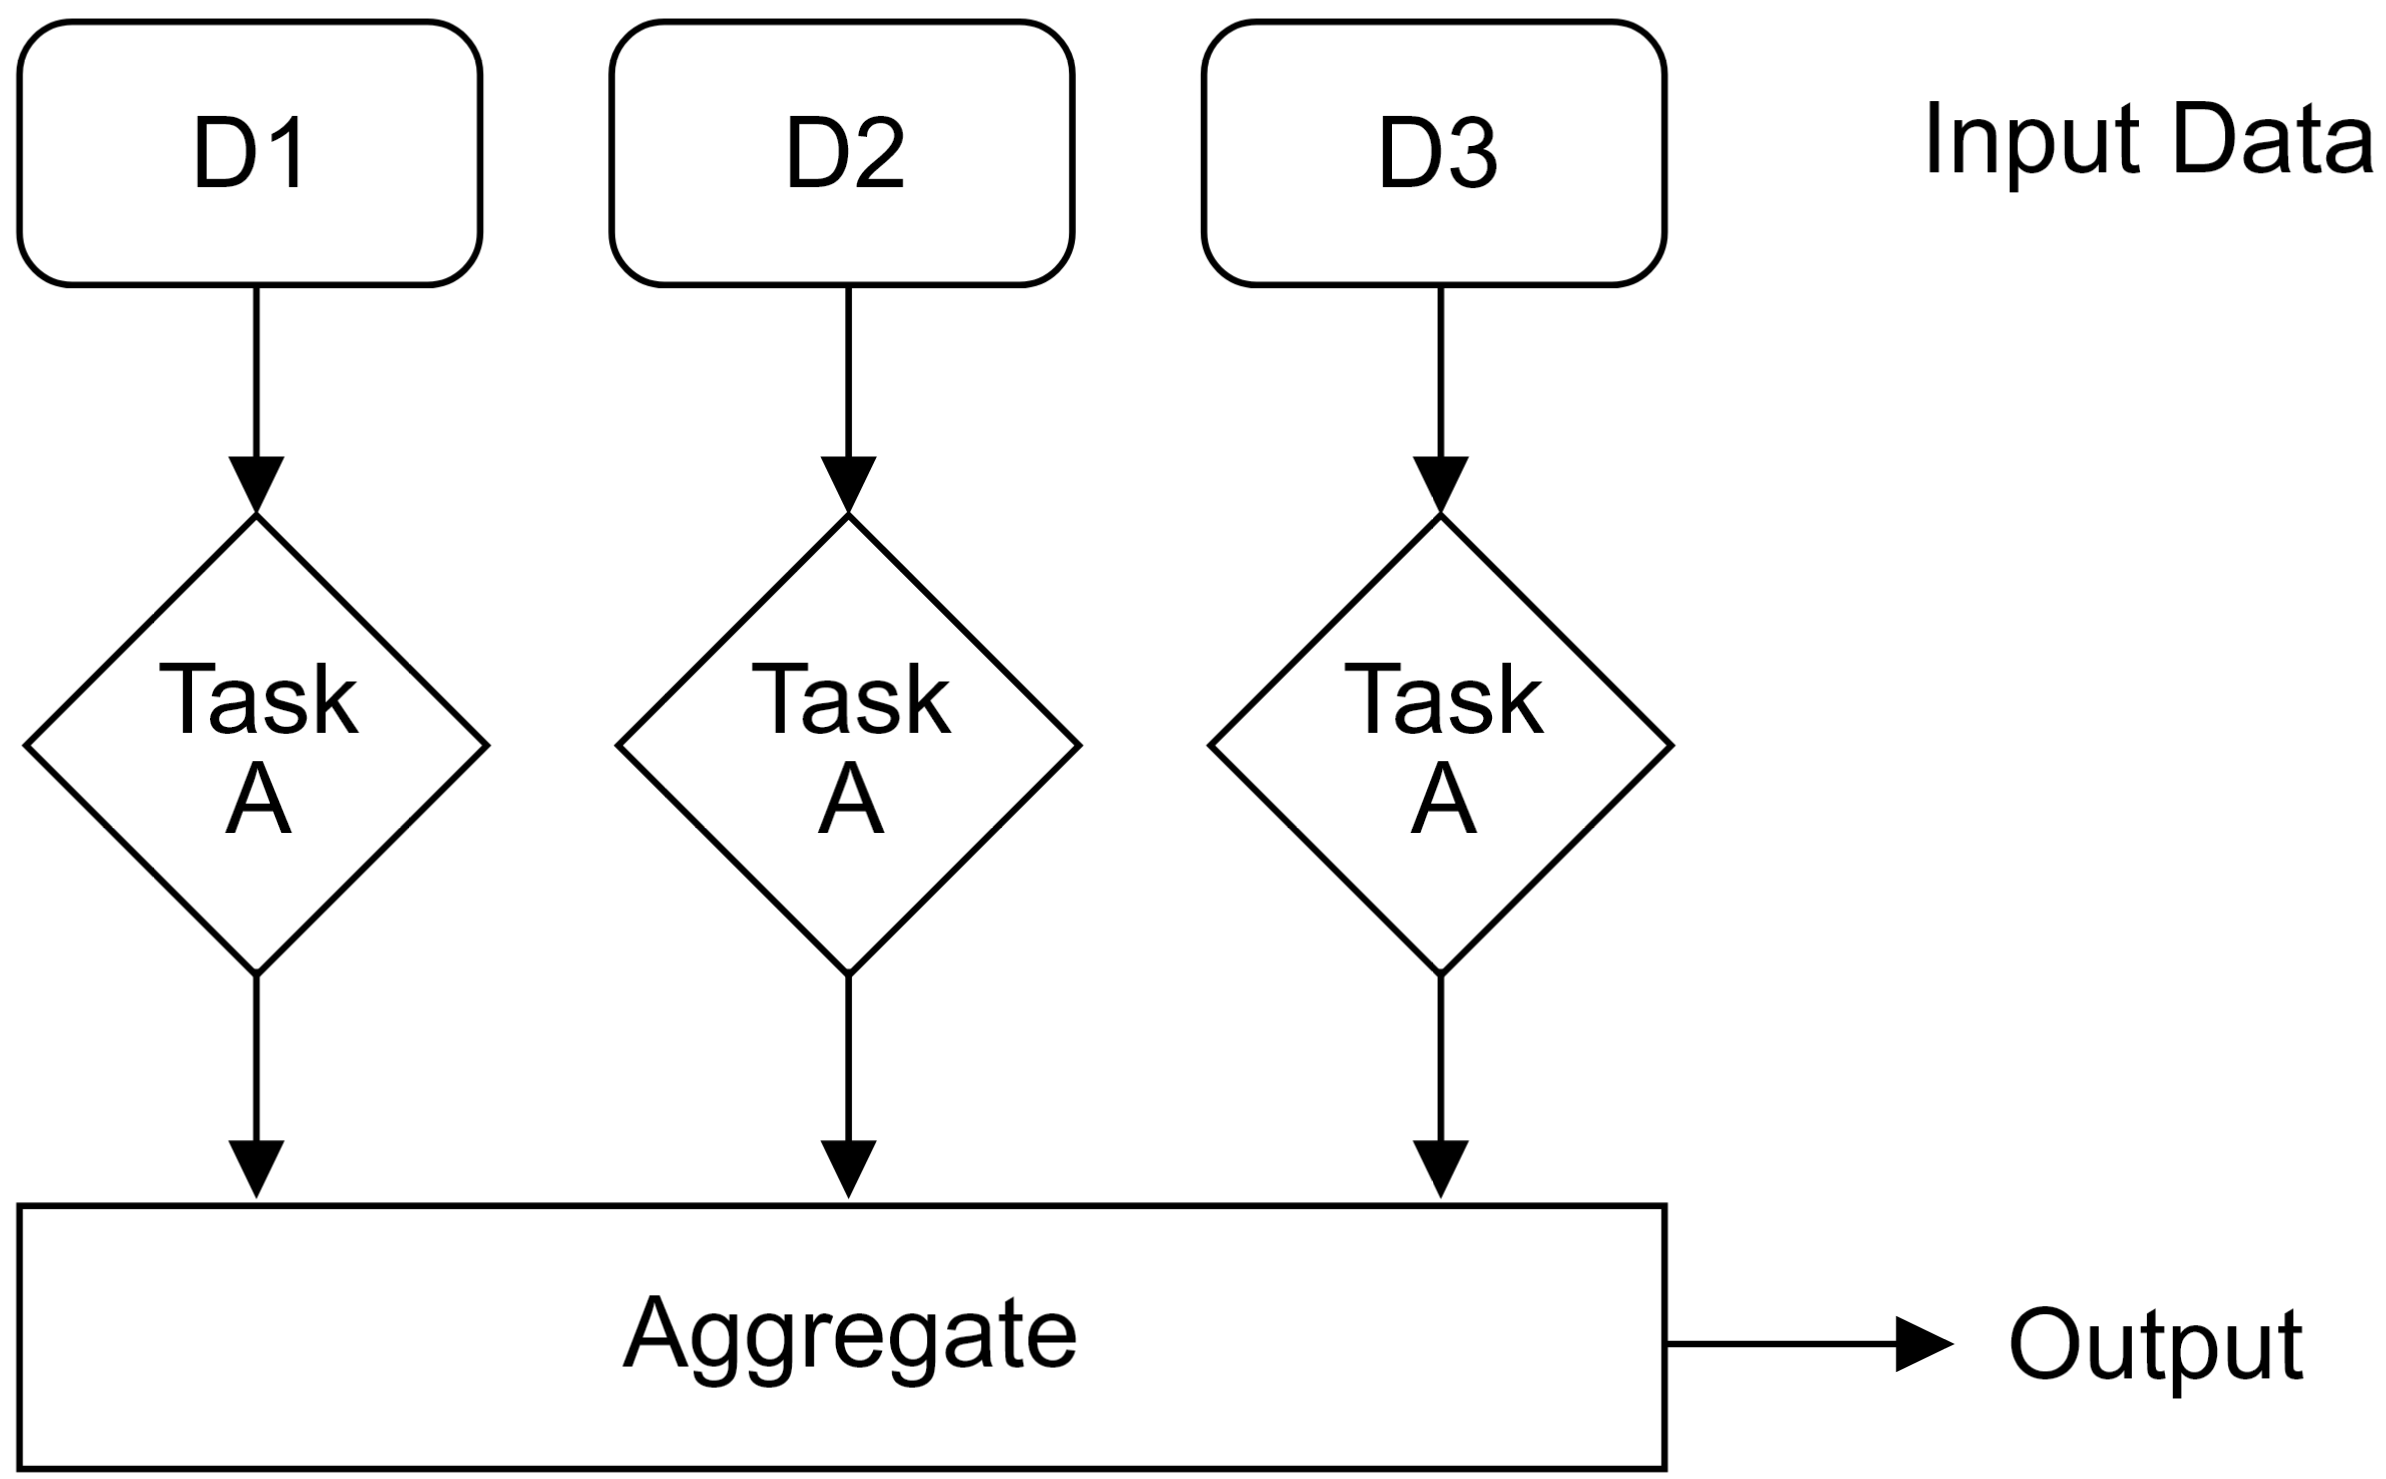
\includegraphics[width=.5\linewidth]{./Sections/rpc_2/dpar.png}\\
\noindent
\rule{\linewidth}{0.4pt}\\
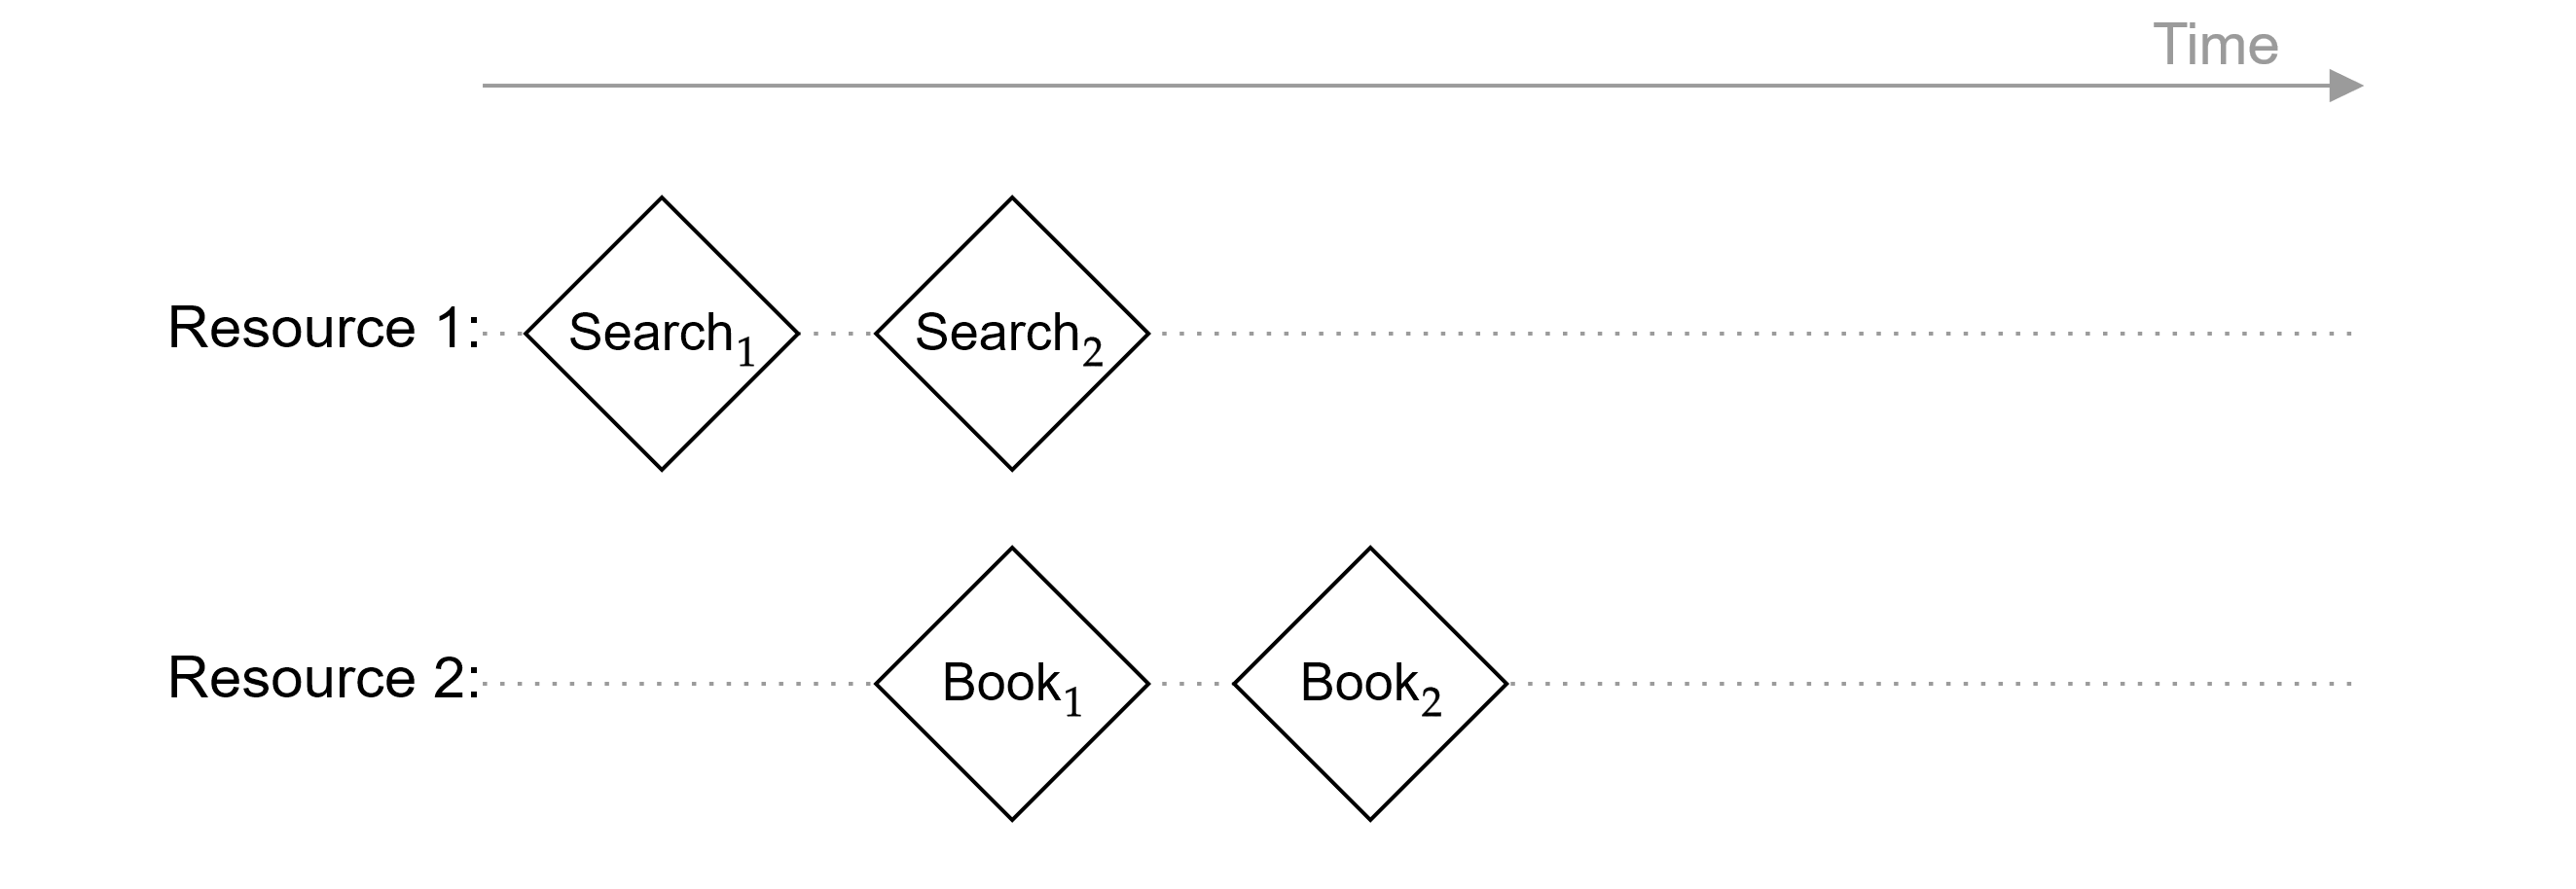
\includegraphics[width=\linewidth]{./Sections/rpc_2/ppar_2.png}
\noindent
\rule{\linewidth}{0.4pt}\\
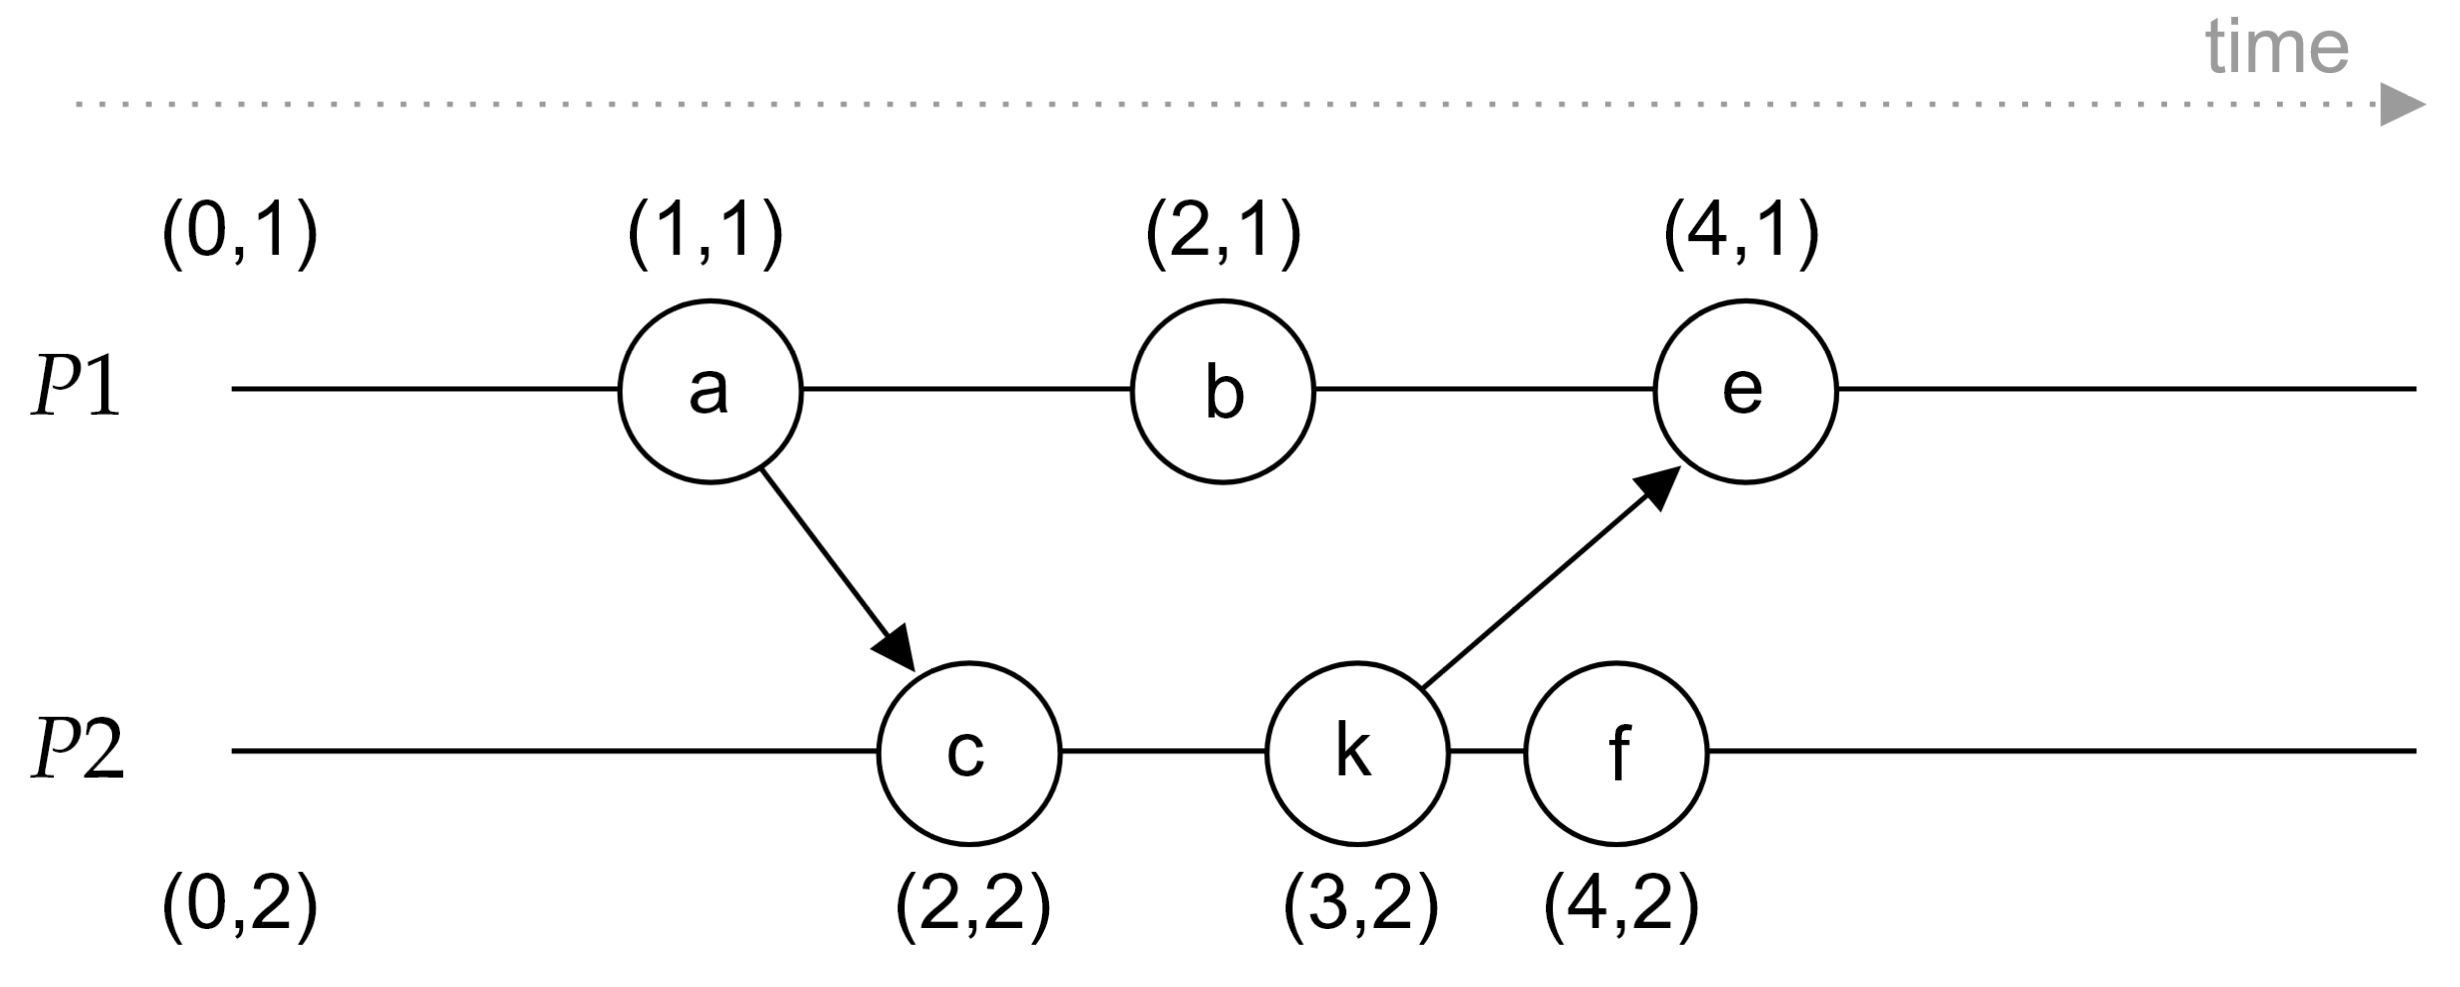
\includegraphics[width=\linewidth]{./Sections/time/lamport.png}
\noindent
\rule{\linewidth}{0.4pt}\\
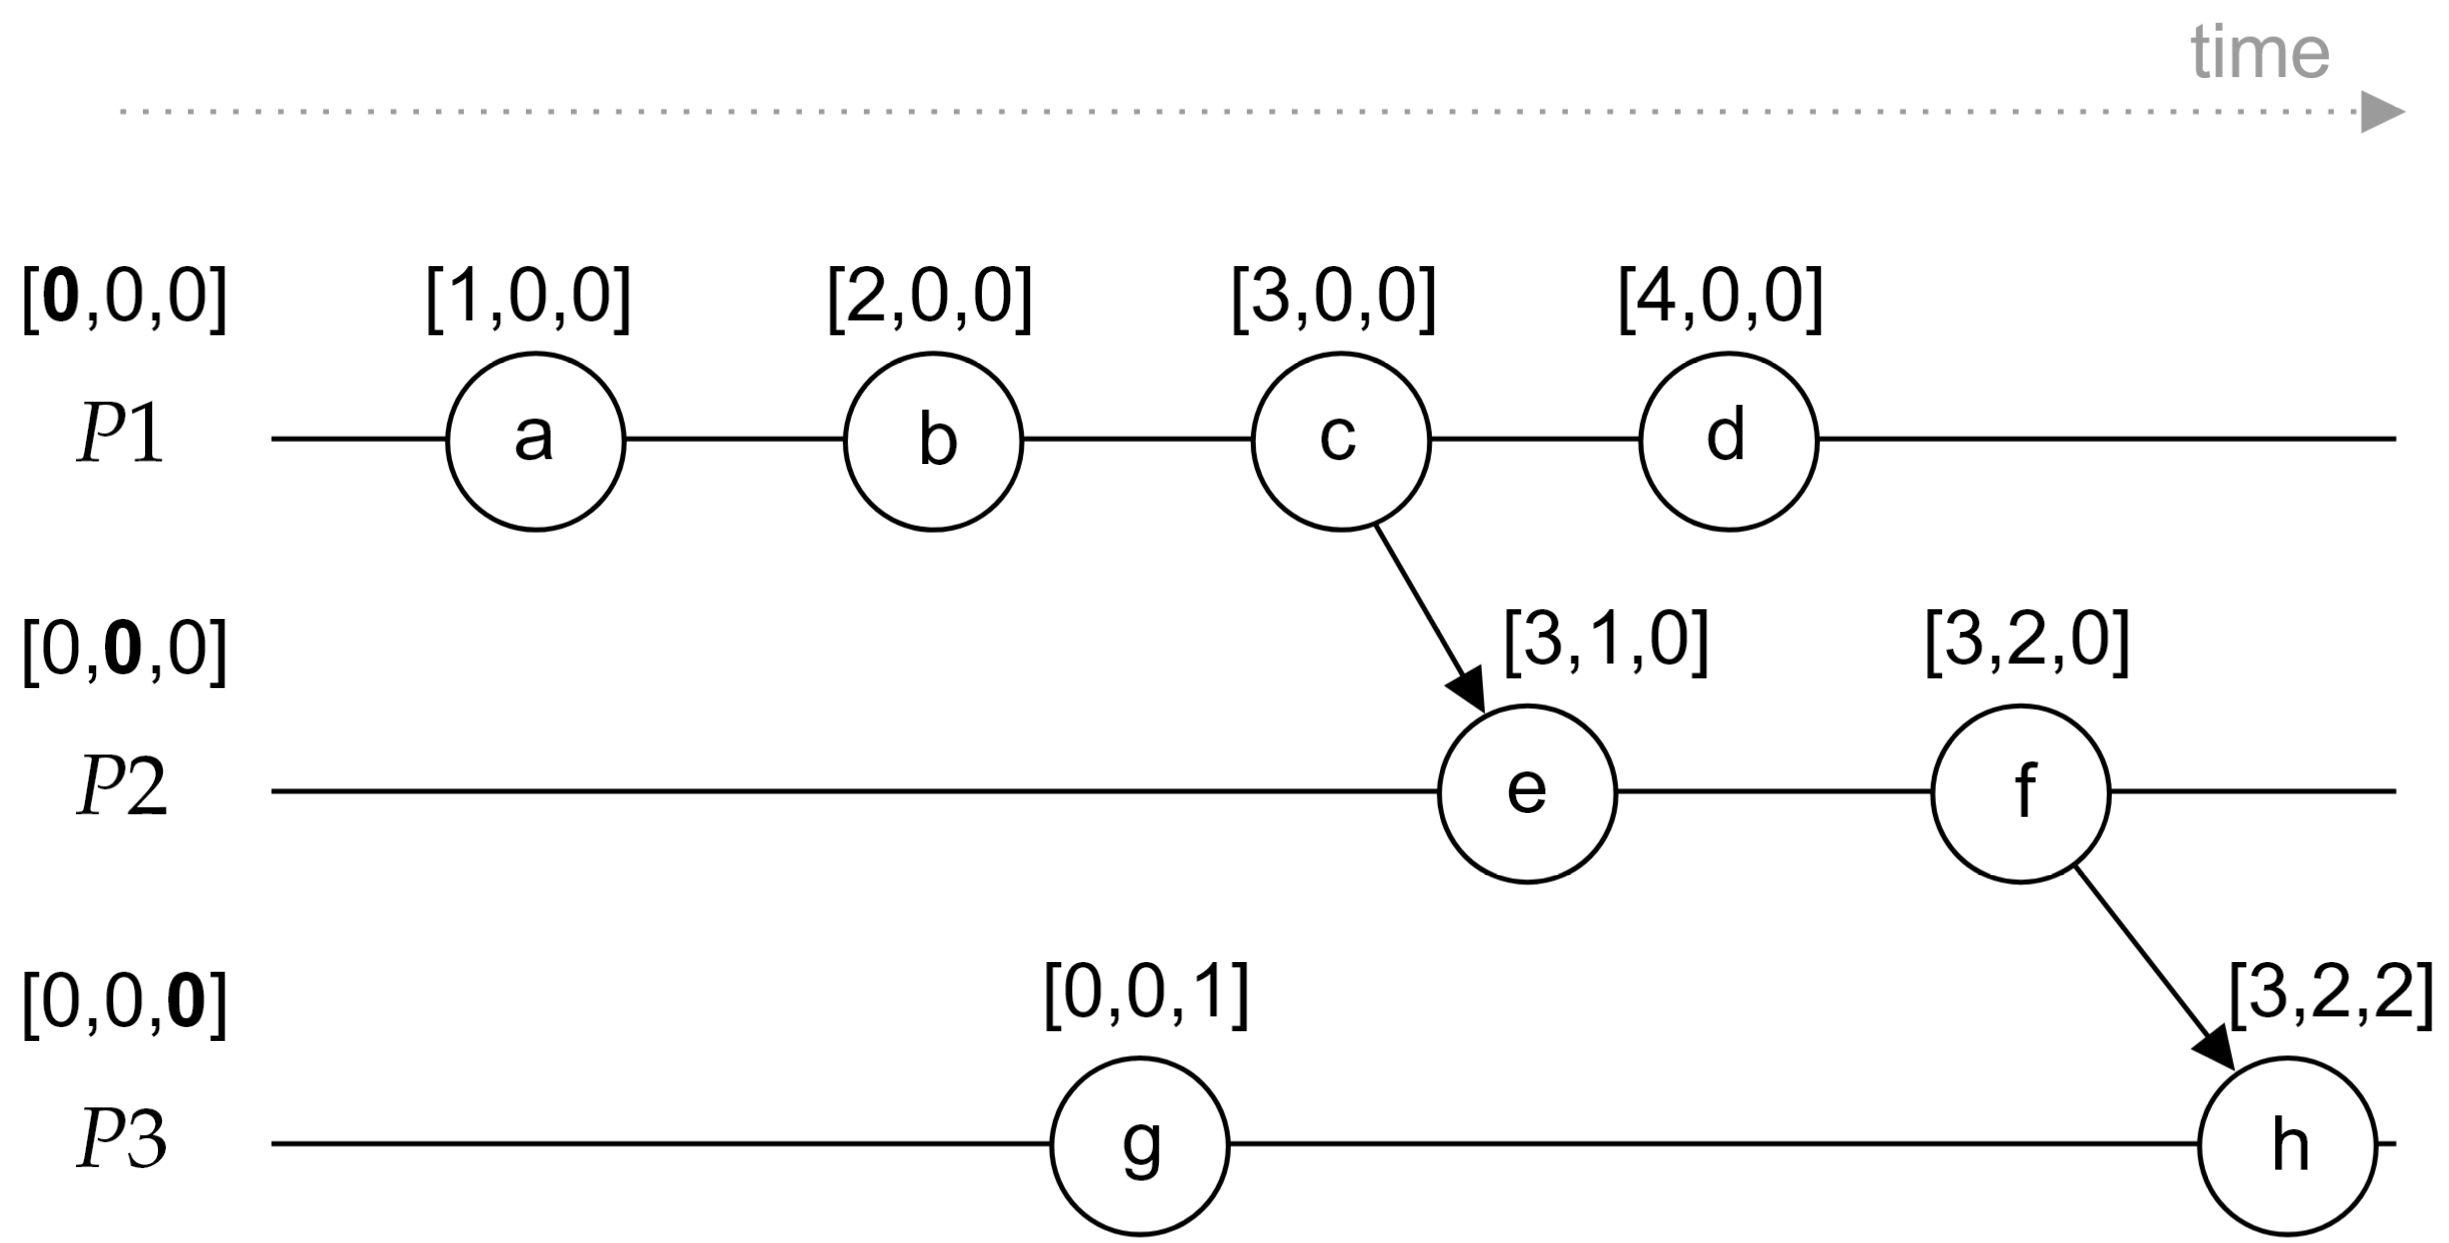
\includegraphics[width=\linewidth]{./Sections/time/vector.png}
\end{multicols}


\newpage

\begin{multicols}{2}
    
    \noindent
    \textbf{Snapshots:} Consistent snap., captures causal dependencies, if 
    $e_1 \to_r e_2$, and $e_2$ is in the snap., $e_1$ must also be present (otherwise it's inconsistent). If in the 
    snap., $e_1$ sent a message to $e_2$, and $e_2$ is not in the snap., replay the message on snap. recovery.
    \textbf{Chandy-Lamp.Snap:} Alg. for capturing consistent snaps. Reqs: No failures, FIFO channels, Strongly conn. graph, Single initiator.
    (1) Marker sent to all out-chans., record local state. (2) On marker retrieval, block (empty) the chan. from which it came. Record local state, except for empty chans. Send marker to all out-chans.
    (3) Completion, When all processes have received and sent a marker, the snapshot is complete.
    (every processes' incoming channel is empty).
    ---\textbf{Replication}---
    \textbf{Def:} Maintaining multiple copies of the same data across distinct nodes (machines), providing fault-tolerance, load-balancing, and availability.
    \textbf{Active vs. Passive Rep:} Active, client sends reqs. to all replicas, must process in FIFO order. Passive, client sends reqs. to one replica (primary), which propagates to others (backups).
    \textbf{State vs. Req. Rep:} State Rep., forwards the entire state to backups. Request Rep., forwards individual reqs. to backups.
    \textbf{Primary Commit:} Client$\to$Primary$\to$Backups$\to$Primary$\to$Client (Commit Point).
    \textbf{Arbitrary Serv. (CFG):} The Configuration Service Provider (CFG) ensures a controlled \textbf{failover} (switching to backups) in the event of a primary failure.
    \textbf{Chain Rep:} An ordered chain of $s_n$ replicas, writes propagate from $s_1$ to $s_n$, where $s_n$ reports back to the client. Reads speak directly with $s_n$. For any failover, the next adjacent successor takes over.
    ---\textbf{Consensus}---\textbf{State Machine:}
    Processes a seq. of inputs from a log, saving them in state. \textbf{Rep. State Machine:} Replicated logs across multiple machines, the processing of 
    which is deterministic, generating the same state.\textbf{Consensus Model:} facilitates agreement of replicated logs between replicas.
    \textbf{Raft:} A consensus algorithm, with a central leader elected by the cluster in monotonically increasing terms. Liveliness is measured by periodic heartbeats, if the leader
    isn't reachable, followers, run for election. Split votes are dealt with the current candidates by timing out again (new timeout). Log Matching Property: Same index and term implies, same command and previous indexes are identical.
    Log Correction: The leader will find the index of the first mismatch, then overwrite the followers entries with its own. Leader Completeness: All proceeding leaders must have all committed entries of the previous leader.
    Leaders may only commit entries from their term. Candidates are rejected if they have a lower term, shorter log. Timings: $heartbeatReceipt \ll electionTimeout \ll failRate$. 
    Cluster Reconfiguration: A joint consensus reconfiguration follows two phases: (1) propagate mix config of old and new, (2) propagate new config, which includes new servers or deletions. New servers
    enter with empty logs. Log Compaction/Snapshotting: Servers independently take snapshots, which truncates all committed logs, storing the last committed log index, term, and state (key-value pairs).
    Clients are always redirected to the leader. 2ReplaysSnap. Primary \& Chain Rep.\\
    \noindent
    \rule{\linewidth}{0.4pt}\\
    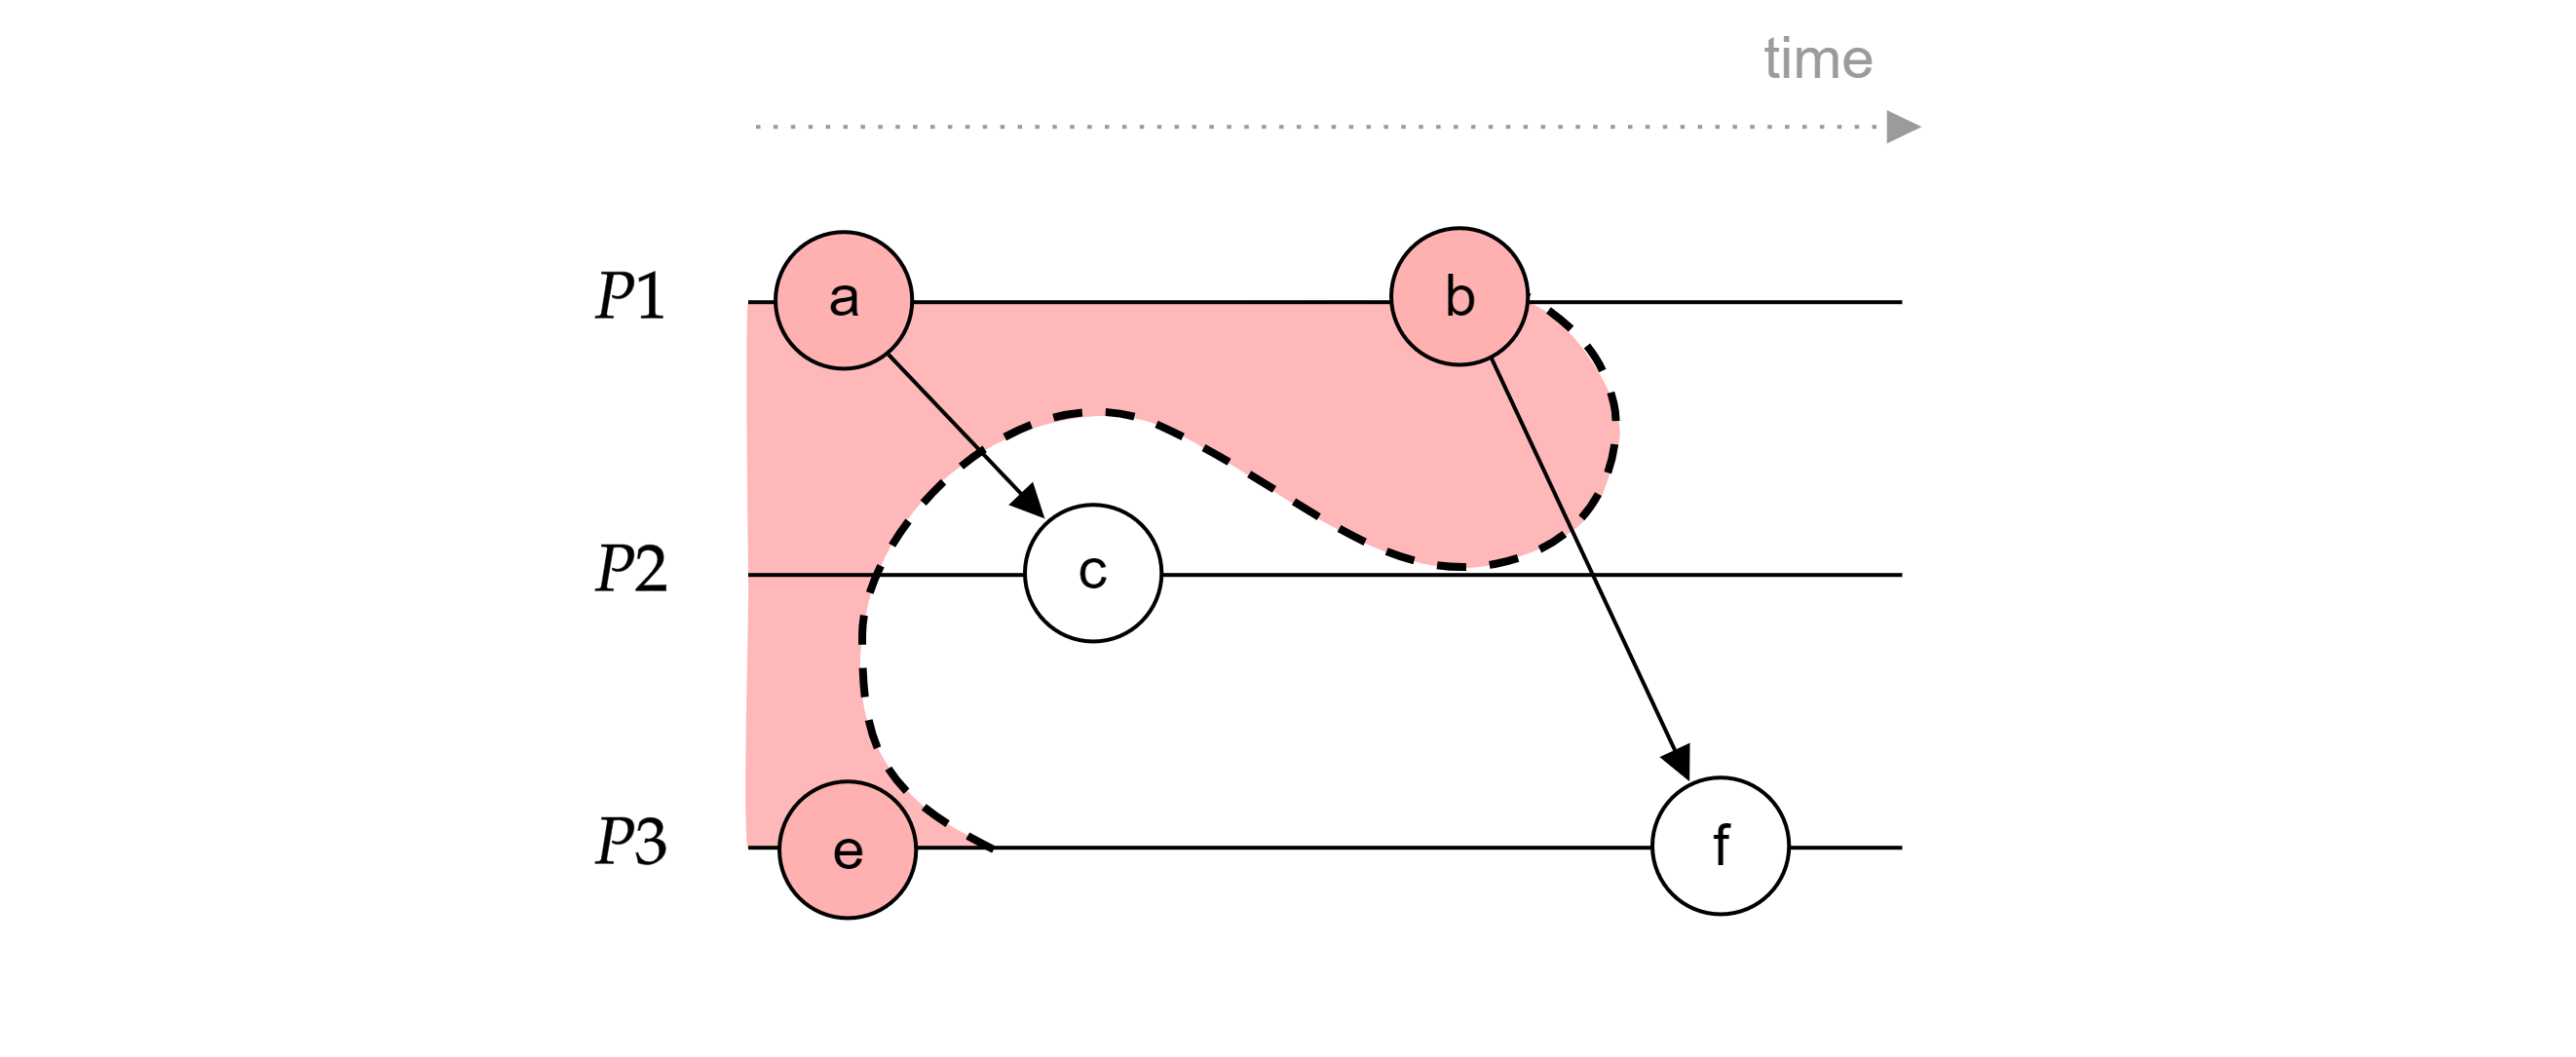
\includegraphics[width=\linewidth]{Sections/snap/snap_2.png}\\
    \vspace{-1.5em}
    \noindent
    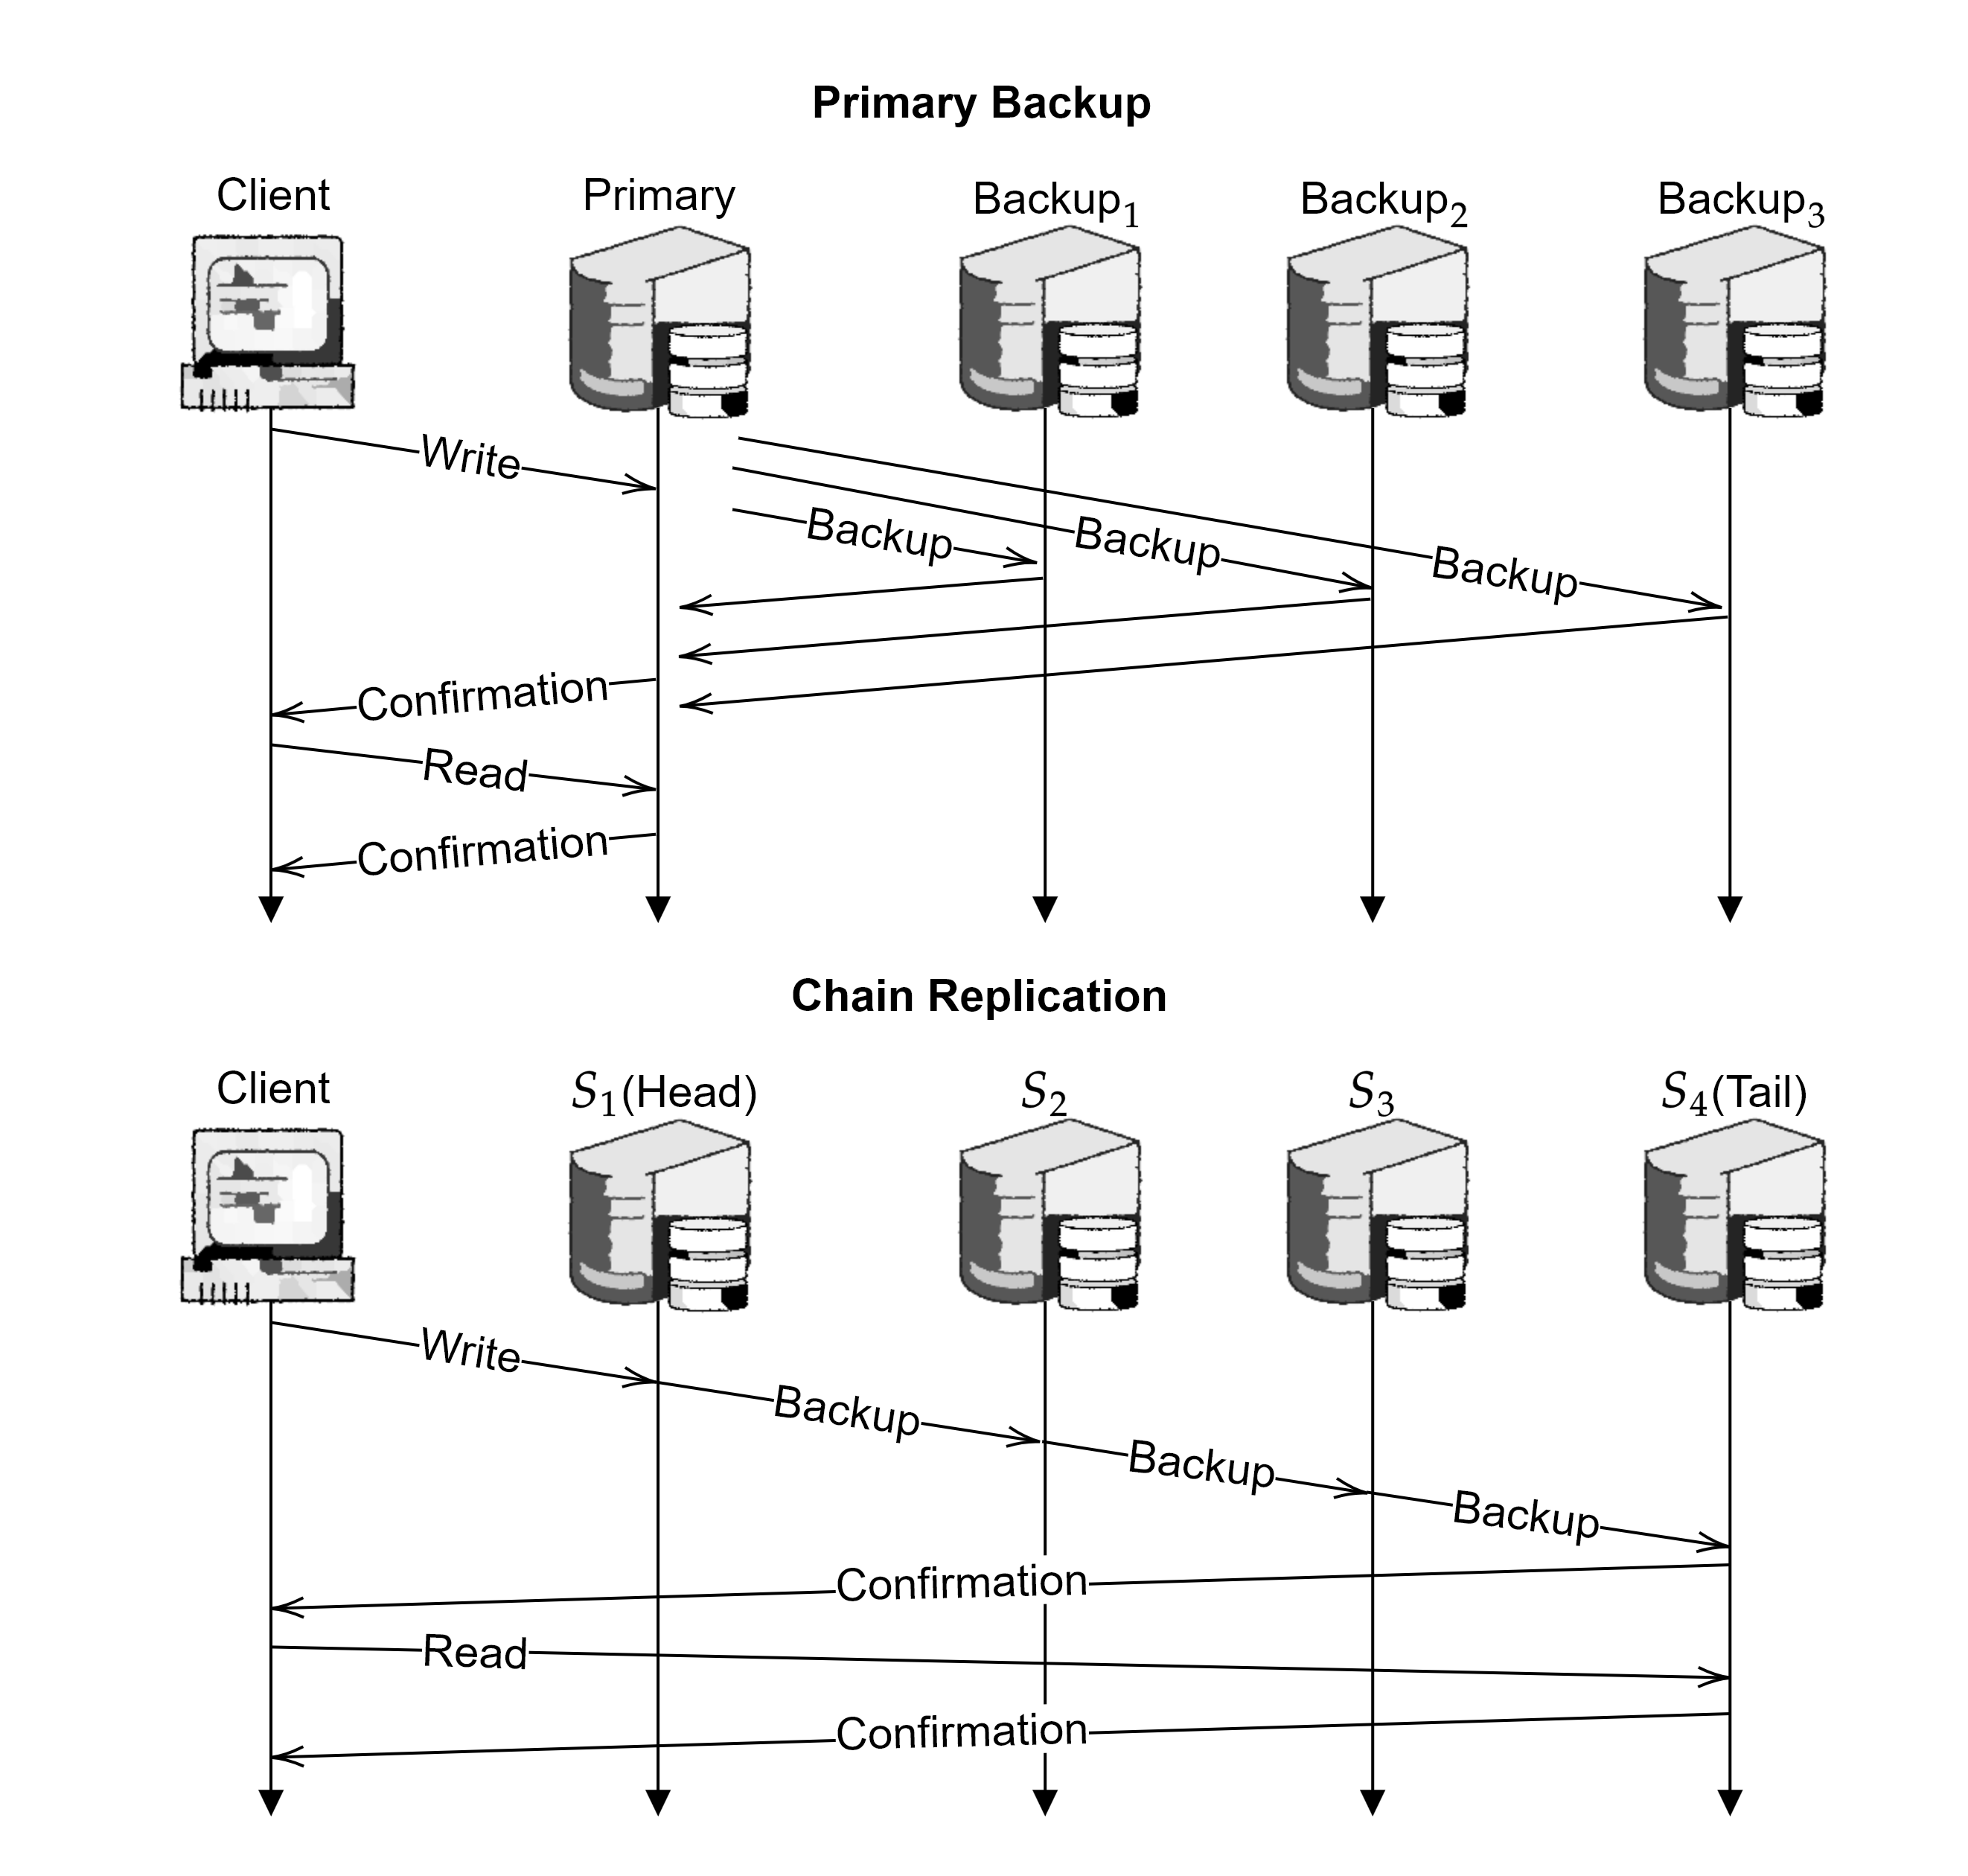
\includegraphics[width=\linewidth]{Sections/rep/comp.png}\\
    
\end{multicols}

\newpage 

\begin{multicols}{2}

\noindent
---\textbf{Failure Model Hierarchy}---Crash-Stop: Process halts, cannot resume (undetectable) $\subset$ Omission: Process fails to properly communicate $\subset$ Crash-Recovery: Process halts, but can recover $\subset$ Byzantine: Process exhibits arbitrary or malicious behavior.
---\textbf{Consistency Models}---\textbf{Def:} A distributed system's method on validating operation orderings on shared data.
\textbf{Global Total Order:} Order of observable events agreed upon by all clients. \textbf{Strong Consistency (Str):} The client observes nodes agree on order execution (all node reads appear to be identical).
\textbf{Weak Consistency (Wck):} The client temporarily observes that nodes disagree on shared data values.
\textbf{Linearizability (Str):} Global Total Order with respect to real-time ordering (operation time intervals unmovable, but execution choice within them are). E.g., Raft leader-commit (happy-path) and Chain Replication.
\textbf{Sequential (Str):} There is some Global Total Order found when shifting operation time intervals.
\textbf{Causal Consistency (Wck):} Same as Sequential; However, clients may observe their own view on a Global Total Order.
\textbf{Eventual Consistency (Wck):} Given no new writes, replicas will eventually agree on the same value after some time.
\textbf{Causal Implications:} Linearizability $\implies$ Sequential $\implies$ Causal $\implies$ (FIFO/RYW).
\textbf{Release Consistency (Wck):} Push updates to all nodes after releasing the lock. 
\textbf{Lazy-release Consistency (Wck):} Push updates to the next node who acquires the same lock.
---\textbf{Transactions}---\textbf{ACID:} Atomicity, no partial effects, all or nothing. Consistency, data departing the database leaves unmutated. Isolation, no interleaving of transactions.
Durability, transactions once committed, are permanent even after system failure.
\textbf{Serializability (Str):} Ensures the outcome of concurrent transactions is the same as if they executed in some serial (sequential) order. Differs from 
linearizability, which deals with real-time ordering of single tasks, as opposed to whole jobs. 
\textbf{Strict-Serializability (Str):} Serializability with real-time ordering; In particular, Serializability $\Longleftarrow$ Strict-Serializability $\implies$ Linearizability.
\textbf{Optimistic Concurrency Control (OCC):} Assumes conflicts are rare, proceeds without locking. (1) Prepare the transaction on all nodes, (2) Tell the coordinator to execute, validate the outcome, (3) Commit if Serializable, abort otherwise (isolation).
\textbf{Timestamping OCC:} Helps with distributed OCC agreement on separated data, but aborts unnecessarily.
\textbf{Two-Phase Commit (2PC):} Ensures atomicity, (1) Prepare Phase: After client's request is received on all nodes, the Transaction Coordinator (TC) sends a prepare message to all nodes, awaiting YES votes. 
(2) Commit Phase: If all nodes reply YES, the TC requests for all nodes to commit. If any fail to reply, the TC is blocked, sending the commit request to that node indefinitely (can't abort after this point).
\textbf{3PC:} 2PC with an additional phase before the commit phase, ensuring people can commit (PreCommit Phase). If any nos or failure to respond in PreCommit, abort. If not 
partitioned, if the TC fails in the PreCommit phase, servers may attempt to reconcile with themselves about how to continue.
\textbf{Pessimistic Concurrency Control (PCC):} Assumes conflicts are likely and prevents them by ac-
quiring locks before any data access. It then preforms actions directly on shared data, ensuring
serializability and isolation. The locks are released after the transaction is completed. 3PC.

\noindent
\rule{\linewidth}{0.4pt}\\

\hspace{-1.5em}
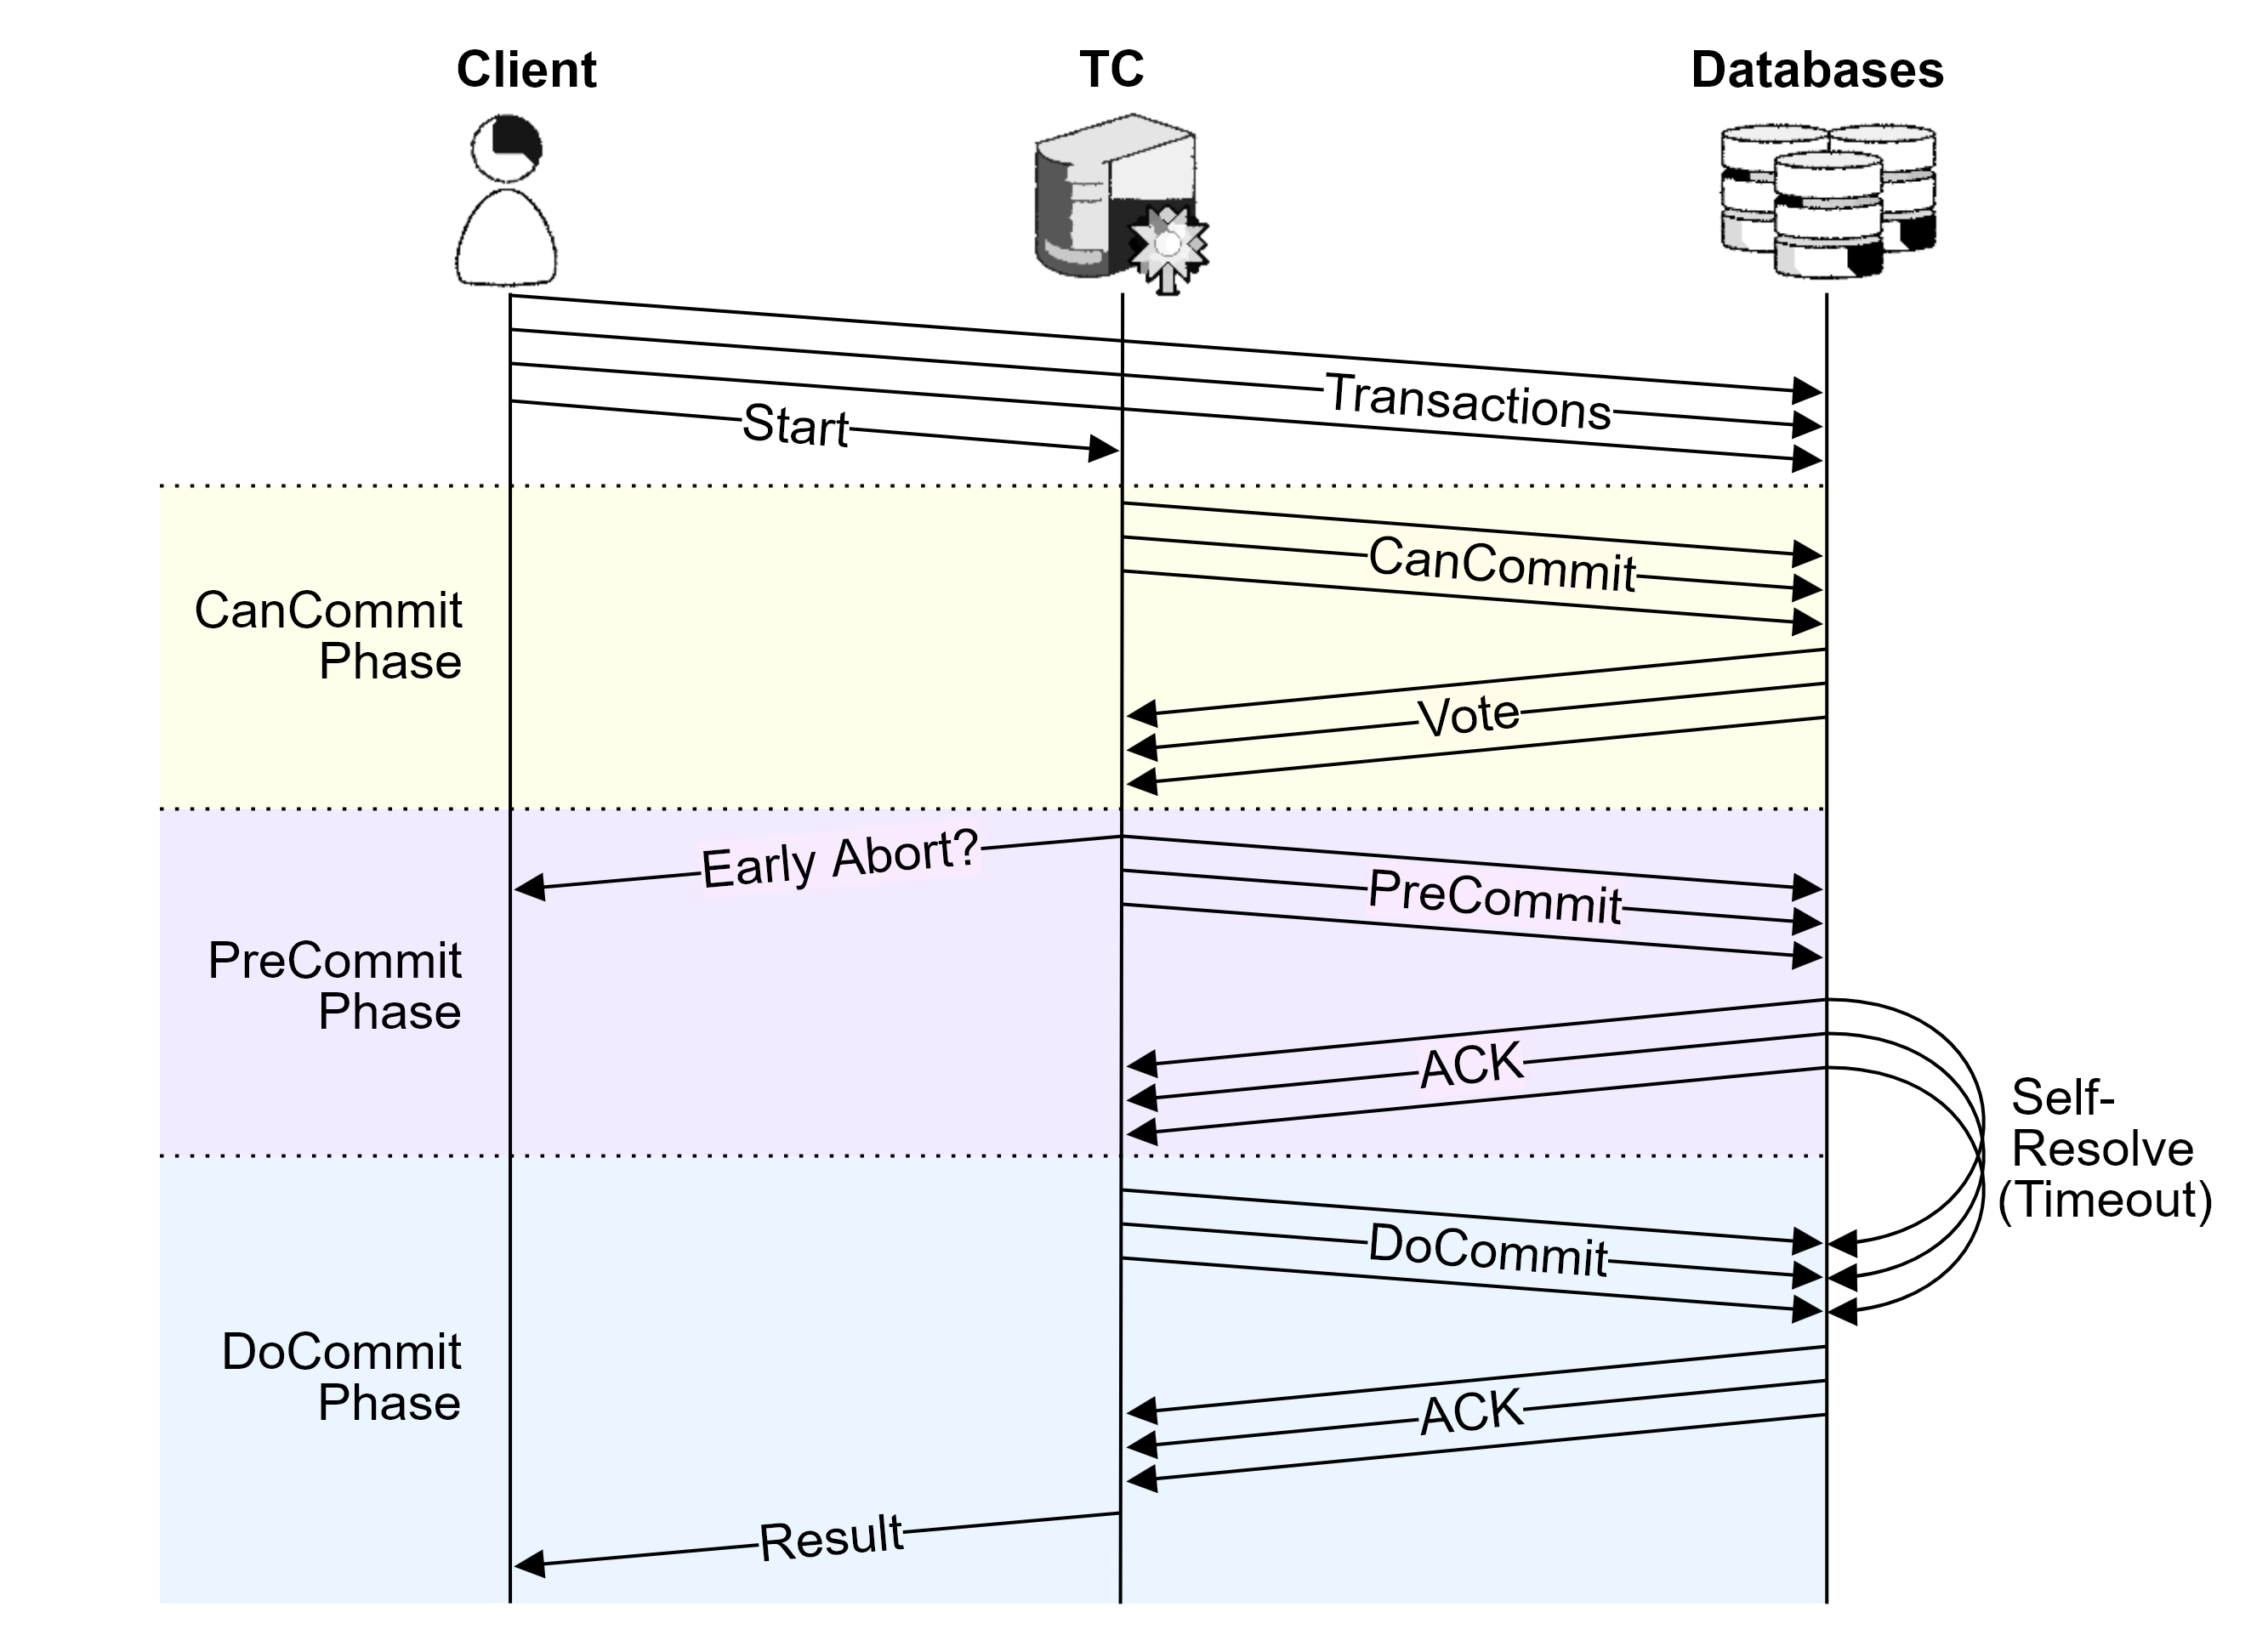
\includegraphics[width=\linewidth]{Sections/trans/3PC.png}\\

\end{multicols}